\subsection{Software design}

\subsubsection{A Road Network}
\label{sec:design:software:network}

The market is represented as a weighted connected graph constructed of edges
(roads) and vertices (origins/destinations). Each vertex has associated
properties: a list of connected edges with their lengths (weights), a list of
passengers, potentially a list of taxis. Each edge has associated properties:
length, potentially speed limit and toll. Taxis can travel between vertices
using edges. Taxis are assumed to take the shortest routes and travel at a
constant speed. Passengers appear at nodes and when taxi is at a node it is
assumed that they can interact, and the passengers wait for a set amount of
time.

Road networks have a specific structure that is different from generic randomly
generated graphs. \textcite{Eisenstat2011graphs+quadtree} believes that the
structure of the graphs is important for optimisation problems, giving the
example of optimising logistics operations for a fleet of vehicles where
algorithmic performance greatly differs from that on generic graphs. Uniform
planar graphs are a reasonably realistic way to represent road networks
\parencite{Eisenstat2011graphs+quadtree, Masucci2009graphs+london}. A way to
generate random planar graphs is suggested by
\textcite{Brinkmann2007graphs+generate}, for which ready-to-use software called
\textit{plantri} is available. 

Shortest paths in graphs can be calculated by Djikstra's algorithm
\parencite{Cormen2009algorithms}. However, calculating all possible shortest
paths is not necessary as some routes could never be travelled. Furthermore,
that may be unfeasible in a very large network as the number of paths grows
exponentially. Online calculation of a shortest path between two nodes in a
graph can be efficiently done using \textit{A-star} algorithm by
\textcite{Hart1968paths}.


\subsubsection{Learning}
\label{sec:design:software:ai}

State is based on the origin, passenger and intended destination. Actions a
taxi can take is enquiring a passenger for destination, offering a price or
driving to another place. If the passenger accepts the price, taxi drives the
passenger to the destination and receives a reward. Keeping track of the exact
passenger is not important. Each time step has a negative reward based on what
action the taxi is taking, always depending on time but also could depend on
distance travelled. The probability of the passenger accepting the fare is the
transition probability. This specifies the research problem as a finite MDP
according to the definition in Section \ref{sec:literature:ai:mdp} (although it
can be argued that prices could theoretically be a continuous space, in reality
they are not).

As described in Section \ref{sec:ai:mdp:methods:advanced}) one of the simplest
solution methods for finite MDP reinforcement learning problems is the basic
temporal difference (TD) learning method. Of course, it needs to be extended to
accomodate exploration in this paricular case of having an active agent.
Temporal difference and its underlying ideas is in the basis of many solution
methods both for MDPs and POMDPs (see Section \ref{sec:ai:pomdp}). Therefore
this approach is the best starting point to examine the research problem on a
small scale. It can later be extended and updated for more complex situations.

The simplest TD implementation is TD(0) \parencite{Russell2010ai+modern}, as
shown in Algorithm \ref{algorithm:td:0}. It can be easily extended to
TD(\lambda) later (Algorithm \ref{algorithm:td:lambda}) by adding eligibility
traces to store some history of experiences. Both of these algorithms introduce
a new concept: the step-size function. This function is used to adjust for the
bias of previous estimates. As a state is being visited more and more, any new
experiences are less and less important compared to the old experiences,
therefore the TD weights should be adjusted less. This issue is discussed in
more detail by \textcite{Sutton1994ai+stepsize}, where three different
algorithms are introduced for optimising the step sizes. However, if the step
size decays (i.e \(\\lim_{n \to \inf}\alpha(n) = 0\) where \(n\) is the number
of times a state has been visited, the policy will still converge. Therefore
for simplicity the function can be fixed as \(\alpha(n)=\frac{1}{n}\).


\begin{algorithm}
  \caption{
  TD(0) Algorithm that needs to be called after each transition. 
  Adapted from \textcite{Szepesvari2010ai+algorithms}
  \label{algorithm:td:0}}

  \begin{algorithmic}[1]
    \Require 
      \Statex $S\_old$ is the last state,
      \Statex $S\_new$ is the next state,
      \Statex $R$ is the immediate reward associated with this transition,
      \Statex $V$ is the array storing the current value function estimate,
      \Statex $H$ is the array storing of the number of times states have
              been visited,
      \Statex $f\alpha$ is the step-size function,
      \Statex $\gamma$ is a discount factor.

    \Function{TD\_basic}{$S\_old,S_new,R,V,z$}
      \State $\delta \gets R + \gamma \cdot V[S\_new] - V[S\_old]$
      \State $V[S\_old] \gets V[S\_old] + \alpha \cdot \delta \cdot z[S\_old]$
      \State $H(S\_new) \gets H(S_\new) + 1$
      \State \Return ($V$)
    \EndFunction
  \end{algorithmic}
\end{algorithm}


\begin{algorithm}
  \caption{
  TD(\(\lambda\)) Algorithm that needs to be called after each transition. 
  Adapted from \textcite{Szepesvari2010ai+algorithms}
  \label{algorithm:td:lambda}}

  \begin{algorithmic}[1]
    \Require 
      \Stetex \chi is the space of all states
      \Statex $S\_old$ is the last state,
      \Statex $S\_new$ is the next state,
      \Statex $R$ is the immediate reward associated with this transition,
      \Statex $V$ is the array storing the current value function estimate,
      \Statex $z$ is the array storing the eligibility traces,
      \Statex $H$ is the visit history of states
      \Statex $\alpha$ is a step-size function,
      \Statex $\gamma$ is a discount factor.


    \Function{TD\_lambda}{$S\_old,S_new,R,V,z$}
      \State $\delta \gets R + \gamma \cdot V[S\_new] - V[S_\old]$
      \ForAll{$x \in \chi$}
        \State $z[x] \gets \gamma \cdot \lambda \cdot z[x]$
        \If{$x = S_\old$}
          \State $z[x] \gets 1$
        \EndIf
        \State $V[x] \gets V[x] + \alpha \cdot \delta \cdot z[x]$
      \EndFor
      \State $H[S\_new] \gets H[S_\new] + 1$
      \State \Return ($V,z$)
    \EndFunction
  \end{algorithmic}

\end{algorithm}


\subsubsection{Software Development}
Ask Nir if this is needed at all?

A paragraph on Kanban? \parencite{Anderson2010kanban}


\subsubsection{Software outline}
\label{sec:design:software}

Expressing the simulation design in Section \ref{sec:design:simulation} and
other software-related considerations discussed in sections
\ref{sec:design:software:network} and \ref{sec:design:software:ai}

Global properties: time; Taxis
can enquire for the route from A to B at a small cost, and receive distance.
When taxis decide to go from A to B, they go at a constant speed for the
calculated time. No actions can be taken and they are marked as travelling.

Network of nodes, not known to taxi as a whole

Node has a list of neighbours and distances.
Node has a list of present passengers and taxis.

Taxi model: fixed cost (per unit of time) and variable costs (per unit of
distance), has a set of actions.

Passenger model: probabilistic properties with set relative weights to
calculate demand, responds to bids with Y/N.

Shown in Figure \ref{figure:design:software}.

\begin{figure}
  \begin{center}
    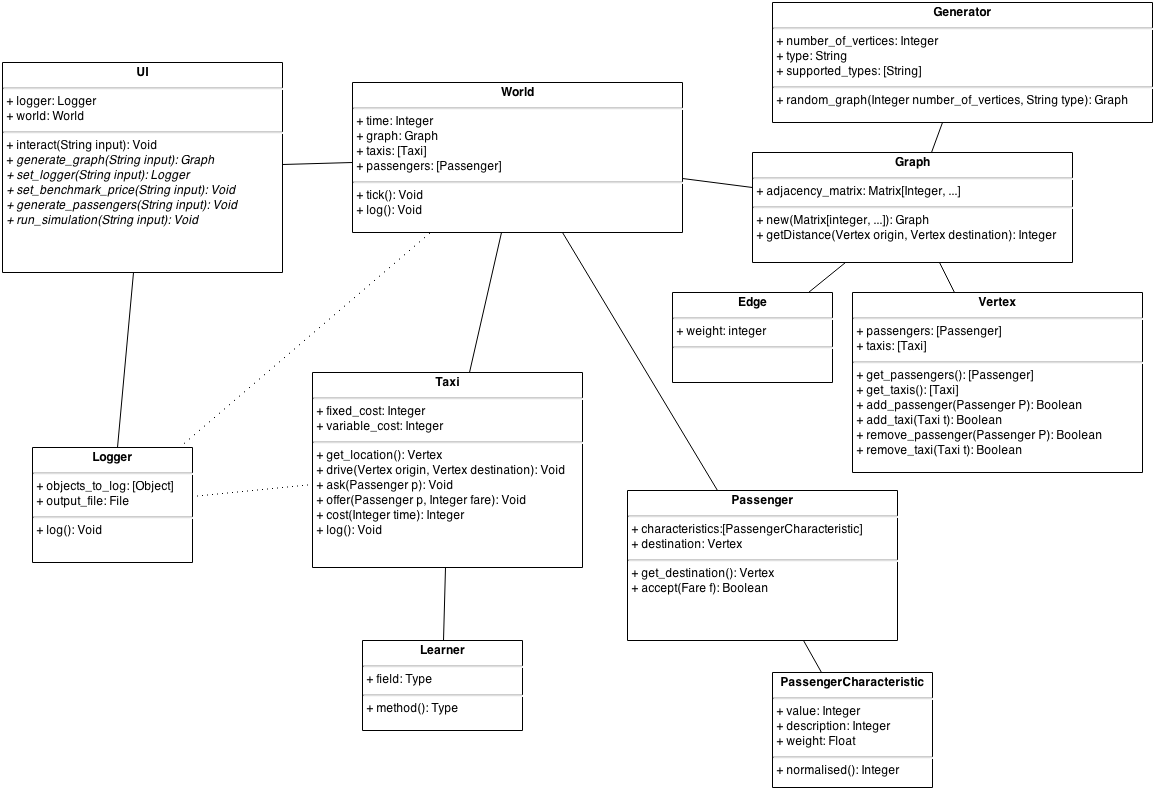
\includegraphics[width=\textwidth]{../figures/software_diagram}
    \caption{
      Software diagram
      \label{figure:design:software}
    }
  \end{center}
\end{figure}
